
\documentclass[12pt]{article}
\usepackage{fullpage,enumitem,amsmath,amssymb,graphicx,url,hyperref}
\usepackage{sectsty}

\hypersetup{
    colorlinks=true,
    linkcolor=blue,
}

\sectionfont{\fontsize{15}{20}\selectfont}

\DeclareMathOperator*{\argmax}{arg\,max}
\DeclareMathOperator*{\argmin}{arg\,min}
\DeclareMathOperator{\E}{\mathbb{E}}
\usepackage{tgpagella}
\usepackage{tcolorbox}
\usepackage{forest}
\usepackage{booktabs}



\begin{document}

\begin{center}
{\Large \textbf{CS224R Spring 2026 Homework 2 \\ Online Reinforcement Learning}}
\\ {\large Due 4/24/2026}

\begin{tabular}{rl}
SUNet ID: & $\hspace{6cm}$\\
Name: & \\
Collaborators: & 
\end{tabular}
\end{center}

\noindent By turning in this assignment, I agree by the Stanford honor code and declare
that all of this is my own work.


\section*{Problem 1: [3 points]}
\subsection*{Your Tasks}

\textbf{Scenario 1} ($r_{\text{step}}=-1$, $R_1=10$, $R_2=5$): Reaches Goal 1. The mild per-step penalty is outweighed by Goal 1's larger reward, making the 7-step path to Goal 1 ($+3$) more valuable than the 4-step path to Goal 2 ($+1$).\\

\textbf{Scenario 2} ($r_{\text{step}}=-2$, $R_1=10$, $R_2=5$): Reaches Goal 2. The doubled per-step penalty makes Goal 1's long path net-negative ($-4$), so the closer Goal 2 ($-3$) becomes optimal.\\

\textbf{Scenario 3} ($r_{\text{step}}=+1$, $R_1=1$, $R_2=1$): Does not reach a goal. Every step yields $+1$ and reaching a goal terminates the episode, so the optimal policy is to never terminate.\\

\newpage


\section*{Problem 2: [3 points]}
 
\textbf{\color{red}Attach a screenshot of the plot \texttt{eval/episode\_success} for this run up to 1 million steps from Wandb. }

\begin{figure}[h]
    \centering
    \includegraphics[width=\linewidth]{}
    \caption{PPO training curve on the hammer task: \texttt{eval/episode\_success} over 1M environment steps.}
    \label{fig:ppo_curve}
\end{figure}

\newpage

\section*{Problem 3: [4 points]}


\noindent\textbf{\color{red}Attach a screenshot of the plot ``eval/episode\_success" for the off-policy run from Wandb up to 100k steps. You should achieve a success rate of at least 90\% before 100K environment steps.}

\begin{figure}[h]
    \centering
    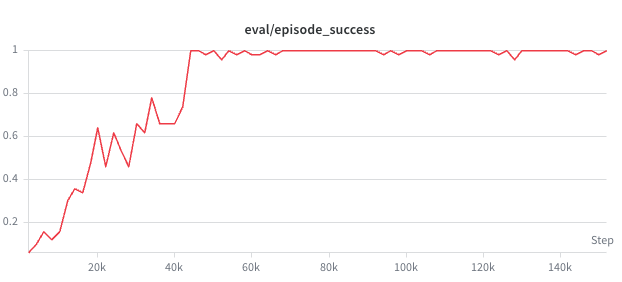
\includegraphics[width=\linewidth]{imgs/off policy.num critics=2,utd=1.png}
    \caption{Off-policy actor-critic (2 critics, UTD=1) training curve: \texttt{eval/episode\_success} over 100k environment steps.}
    \label{fig:utd1_curve}
\end{figure}

\newpage



\noindent\textbf{\color{red}Attach a screenshot of the plot ``eval/episode\_success" for the off-policy UTD 5 run up to 40k steps and compare it to the previous question. Provide a brief, one-sentence explanation of why we observe these effects.}

\begin{figure}[h]
    \centering
    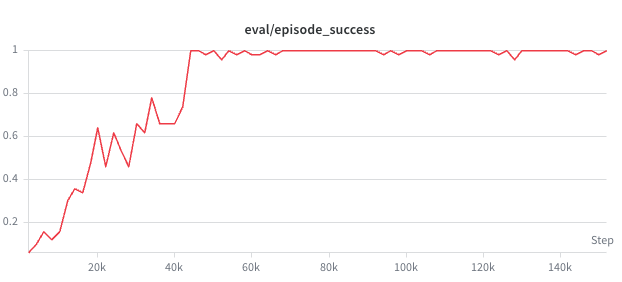
\includegraphics[width=\linewidth]{imgs/off policy.num critics=2,utd=1.png}
    \caption{Off-policy actor-critic (10 critics, UTD=5) training curve: \texttt{eval/episode\_success} over 40k environment steps.}
    \label{fig:utd1_curve}
\end{figure}

\newpage



\noindent Compare the PPO learning curve (\texttt{eval/episode\_success}) from Problem 2 with the actor-critic curve from Problem 3 (2 critics, UTD=1). \\
 
\noindent \textbf{\color{red}In 3--5 sentences, explain at least two concrete differences you observe between the two algorithms in terms of sample efficiency and final performance. Justify each observed difference by connecting it to a specific property of each algorithm.}



%\bibliography{Homework1/references}
%\bibliographystyle{unsrt}

\end{document}
